\chapter{Methodology}
\label{chap:methodology}

\graphicspath{{figs/methodology/}}

\section{Point Cloud Data}
\label{sec:point_cloud_data}

This project aims to work with large amounts of point cloud data. They contain arrays of three-dimensional coordinates and four-component color data. The color information does not affect performance strongly. However, the massive number of points itself introduces a heavy load on computer resources. For improving the performance of visualization software, this work proposes two methods: Generating Levels of Detail (LODs) and Creating a mesh.


\section{Data Preprocessing}
\label{sec:data_preprocessing}

The data themselves are stored in a VLP-16 PCAP file as captured packet stream from a lidar. Therefore, it is necessary to preprocess original files before working on the point cloud. The preprocessing involves three main steps: converting the file from PCAP format to the LAS format, importing the LAS file into Unity, and splitting the point cloud data into chunks.

Converting the PCAP files to the LAS format and importing them into Unity are covered in the \autoref{chap:implementation}.

\subsection{Splitting into chunks}

For the proposed methods, it is crucial to split the point cloud into smaller units (chunks) that are easier to process. It also allows processing the data in a parallel manner, thereby making the algorithms more scalable in terms of performance.

In terms of the Innopolis Simulator project, the chunk is a space bounded by the computed borders. A chunk has a position and a size, which is the same for its width, height, and depth.

As a part of this project, we developed an algorithm for splitting the data into chunks. At the start, the algorithm computes the number of chunks in three dimensions using the \autoref{eqn:n_chunks}. It uses the predefined chunk size and the boundaries of the point cloud object.

The number of chunks for an axis $\alpha$ is computed as follows ($BBox$ stands for boundnig box):

\begin{equation}
\label{eqn:n_chunks}
N_{chunks}^\alpha = \lceil BBox_{max}^\alpha - BBox_{min}^\alpha \rceil / Size_{chunk}
\end{equation}

The chunk grid has the size of $N_{chunks}^X \times N_{chunks}^Y \times N_{chunks}^Z$. The chunks are stored in a three-dimensional array. It means that each chunk has its corresponding index.

After that, the algorithm iterates over all points and computes the exact chunk index they correspond to, based on their global position.

The chunk index for a point with position $pos$ on an axis $\alpha$ is computed as shown in formula \ref{eqn:point_index} using the bounding box ($BBox$ coordinates):

\begin{equation}
\label{eqn:point_index}
Index_{pos}^\alpha = \left \lfloor \frac{pos^{\alpha} - BBox_{min}^\alpha}{Size_{chunk}} \right \rfloor
\end{equation}

Finally, the points are stored within chunks. It is now possible to read the point cloud data in chunks.


\section{Method 1: Generating LODs}
\label{sec:generating_lods}

The level of detail defines the complexity of the model \cite{Luebke2002}. For this project, the level of detail adjusts the number of points shown for a particular object.
The LOD of L shows $L\%$ of all object points. For example, a chunk with LOD 100 contains all its points, while a chunk with LOD 75 has $75\%$ of its points.

\begin{figure}[h]
    \centering
    
    \begin{subfigure}{0.2\textwidth}
        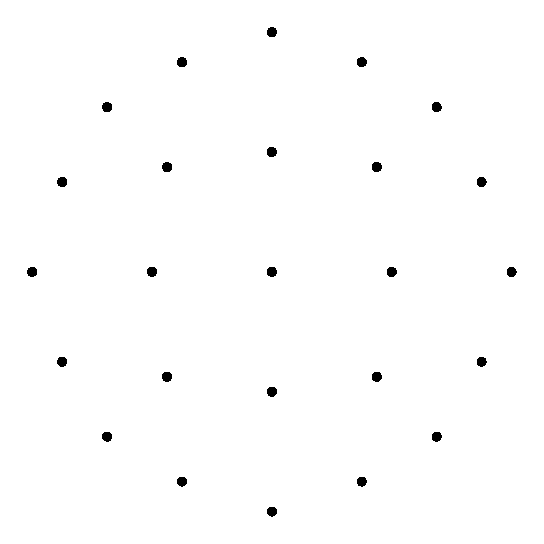
\includegraphics[width=\textwidth]{lod-cloud-25.pdf}
        \caption{$LOD = 25$}
    \end{subfigure}
    % side-by-side
    \begin{subfigure}{0.2\textwidth}
        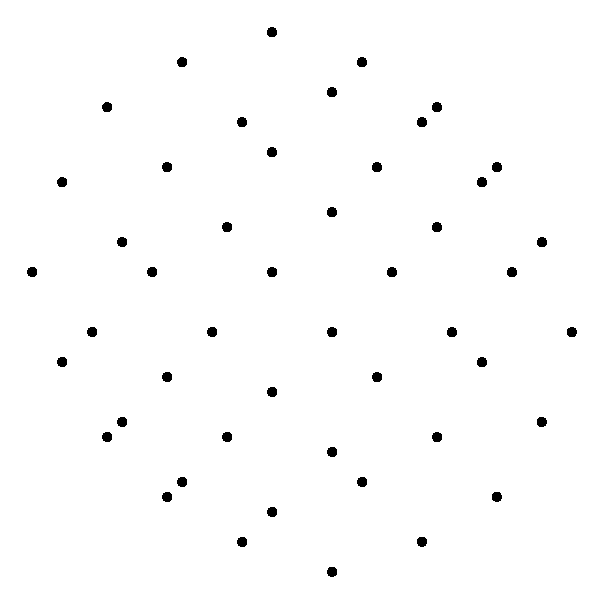
\includegraphics[width=\textwidth]{lod-cloud-50.pdf}
        \caption{$LOD = 50$}
    \end{subfigure}
    % side-by-side
    \begin{subfigure}{0.2\textwidth}
        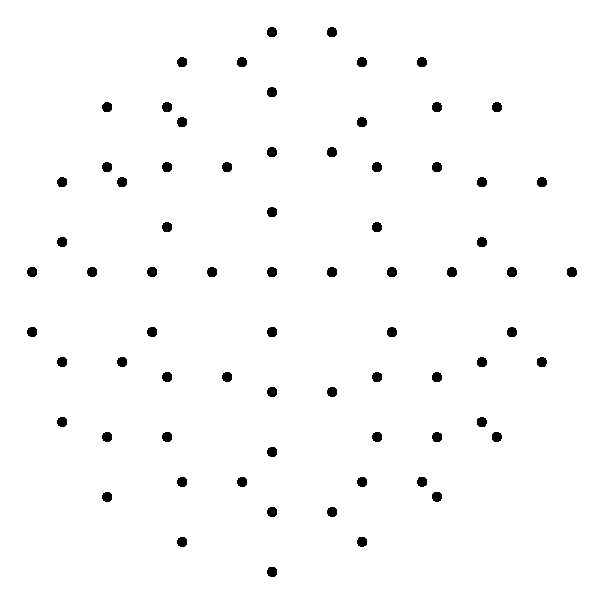
\includegraphics[width=\textwidth]{lod-cloud-75.pdf}
        \caption{$LOD = 75$}
    \end{subfigure}
    % side-by-side
    \begin{subfigure}{0.2\textwidth}
        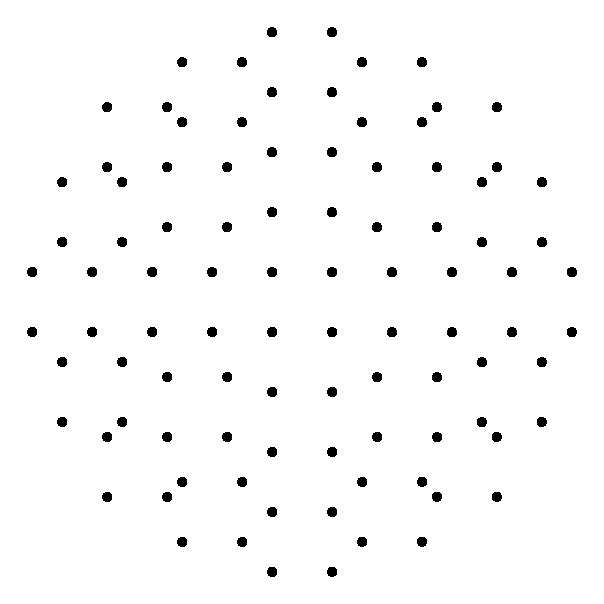
\includegraphics[width=\textwidth]{lod-cloud-100.pdf}
        \caption{$LOD = 100$}
    \end{subfigure}
    
    \caption{Different LODs of a point cloud.}
    \label{fig:cloud_lods}
\end{figure}

The approach is to generate different levels of detail for each chunk, so it will be possible to show fewer points for chunks that are far enough, and thus, are not likely to be noticed.

\subsection{Reducing the number of points}

When loading the data with a specific LOD, the algorithm takes each $stride^{th}$ element from the set of all chunk points. Stride is calculated using \autoref{eqn:lod_stride}.

\begin{equation}
\label{eqn:lod_stride}
stride(LOD) = \frac{100}{LOD}
\end{equation}

\begin{figure}[htb]
    \centering
    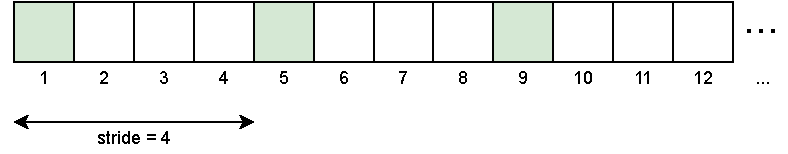
\includegraphics[width=0.8\textwidth]{lod-stride.pdf}
    \caption{Example of stride with $LOD = 25$. In this case $stride(25)=4$.}
    \label{fig:stride}
\end{figure}

\begin{algorithm}
    \caption{Picking points with stride.}
    
    int i $\gets$ 0\;
    Point[$\;$] newPoints $\gets$ [$\;$]\;
    \For{p in points}{
        \If{i \% stride == 0}{
            newPoints.add(p)\;
        }
    }
\end{algorithm}

Different levels of detail are pregenerated for each chunk. The algorithm generates distinct assets\footnote{Asset is an item that can be used within an application (3D model, picture, audio, code, etc.).} for each requested LOD.

When visualization is in progress, the LOD for each chunk is selected based on the distance between the viewer and the chunk. A user predefines the distances and corresponding LODs. The distance between two objects can be computed using the Pythagorean theorem (\autoref{eqn:pythagorean_3d}) as the coordinates are available for all objects.

\begin{equation}
\label{eqn:pythagorean_3d}
distance(p_1, p_2) = \sqrt{(p_1^x-p_2^x)^2 + (p_1^y-p_2^y)^2 + (p_1^z-p_2^x)^2}
\end{equation}

\subsection{Time complexity}

This algorithm traverses all chunk points once, so the complexity can be evaluated as $\mathcal{O}(n)$ (where $n$ is the number of points in a chunk), assuming that copying a point has constant complexity.


\section{Method 2: Creating a Mesh}
\label{sec:creating_mesh}

Mesh is a data structure that contains vertices, texture data, normals, and other details \cite{UnityScriptingMesh}. Later, when a graphical engine visualizes the data, the engine combines the mesh data and draws the mesh on the scene.

Mesh creation consists of several stages:

\begin{enumerate}
    \item Map the point cloud into a grid.
    \item Generate triangles.
    \item Fill the mesh.
\end{enumerate}


\subsection{Vertex grid}

Meshes consist of vertices, and the algorithm first creates a set of vertices that later form the mesh.

For that, the algorithm generates a flat grid of vertices. It is a square-bounded grid-aligned region that has a specified side length. It has $side length \times side length$ dimensions. Each point of this plane has a height value initially set to zero.

\begin{figure}[ht]
    \centering
    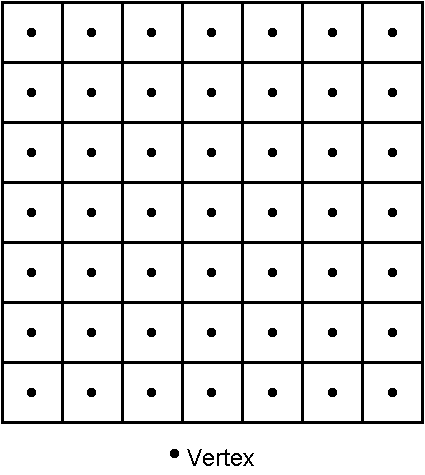
\includegraphics[width=0.3\textwidth]{vertex-grid.pdf}
    \caption{Vertex grid}
    \label{fig:vertex_grid}
\end{figure}


\subsection{Mapping the point cloud into the grid}

\subsubsection{Occurrence map}

The algorithm fills the occurrence map to determine where the mesh triangles should appear. The \textit{occurrence map} tracks the presence of points within the specified grid cells. Also, it has the same size as the vertex grid. Initially, all map values are set to false. It means that no points have been noticed here yet. Further, the algorithm maps each point within a chunk to a specific occurrence map cell. Thus, the occurrence map represents a strictly aligned version of the point cloud viewed from above.

\begin{figure}[ht]
    \centering
    
    \begin{subfigure}[t]{0.3\textwidth}
        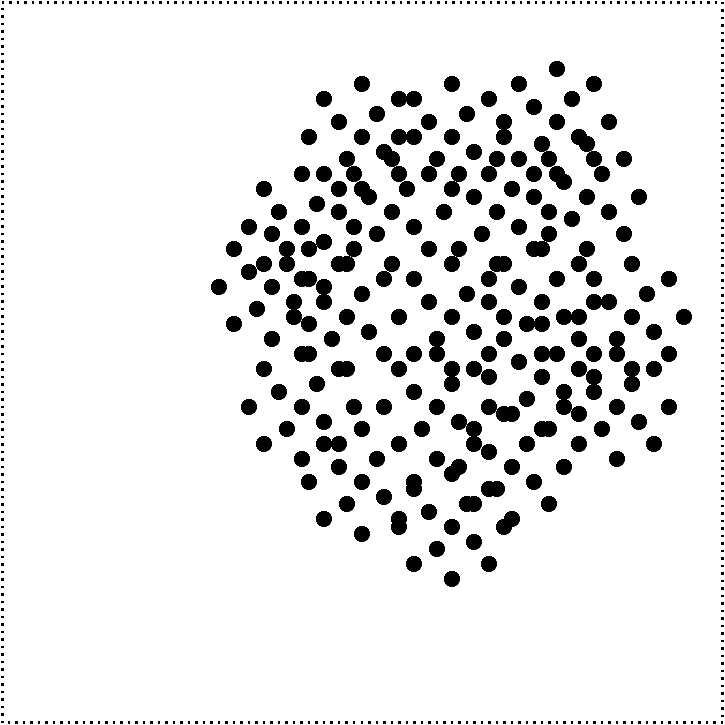
\includegraphics[width=\textwidth]{point-cloud-plot.pdf}
        \caption{Example of point cloud data in two dimensions.}
    \end{subfigure}
    % side-to-side
    \begin{subfigure}[t]{0.3\textwidth}
        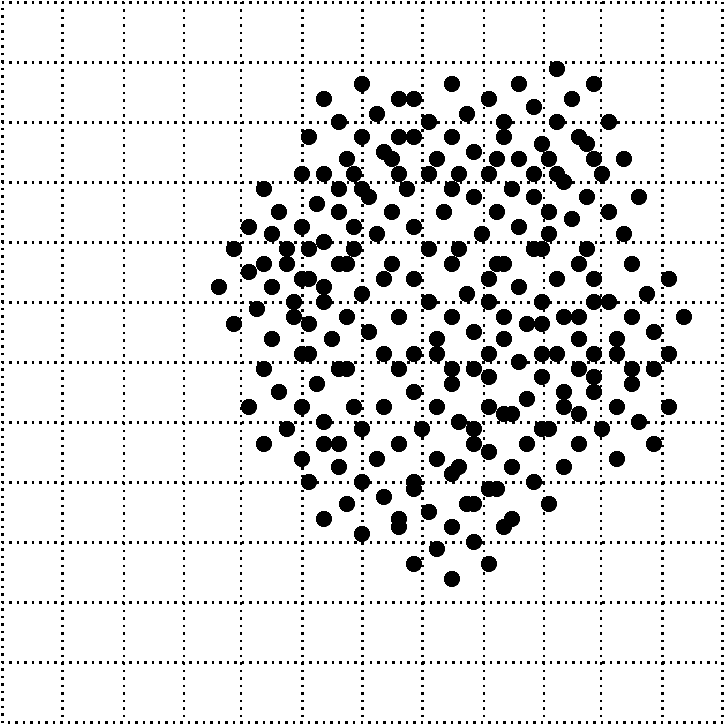
\includegraphics[width=\textwidth]{occurrence-grid.pdf}
        \caption{Occurrence grid.}
    \end{subfigure}
    
    \begin{subfigure}[t]{0.4\textwidth}
        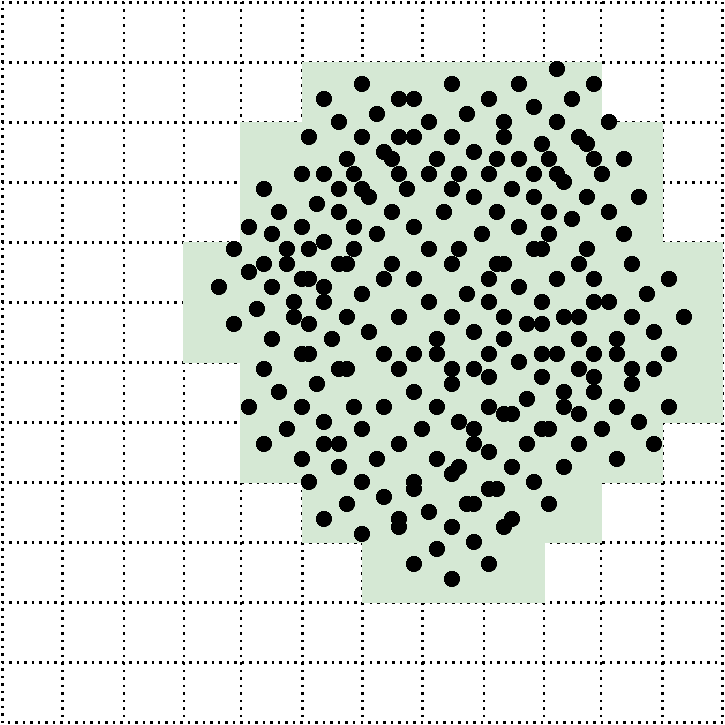
\includegraphics[width=\textwidth]{occurrence-map-applied.pdf}
        \caption{Applied occurrence map.}
    \end{subfigure}
    
    \caption{Applying occurrence map.}
    \label{fig:occurrence_map}
\end{figure}


\subsubsection{Calculating cell indices}

To correctly position points within the grid, the algorithm should calculate a cell index for each point.

To calculate the index, it should do the following (\ref{eqn:cell_coordinate}):
\begin{enumerate}
    \item Calculate a local coordinate within chunk.
    \item Divide the local coordinate by cell size.
    \item Truncate the result down.
\end{enumerate}

\begin{equation}
\label{eqn:cell_coordinate}
Cell\:coordinate(p) = \left \lfloor \frac{Pos(p) - chunk origin}{cell size} \right \rfloor
\end{equation}


\subsection{Traversing points and emitting new vertices}

After initializing the vertex grid and occurrence map, the algorithm starts processing the point cloud itself.

For each point in a point cloud, the algorithm  calculates its grid cell index and fills the corresponding cell in the vertex grid and occurrence map.

At the vertex grid, the algorithm compares the height value stored in the cell and the height of the point (its $Y$ coordinate). If the value stored in the grid is less than the point height, the algorithm writes the point height to the grid cell.

At the occurrence map, the algorithm tracks the occurrence of the points in the grid cells. If a point belongs to the cell, that cell is marked as visited.


\begin{algorithm}
    \caption{Filling the vertex grid and occurrence map.}

    \For{point \textup{p} in \textup{points}}{
        x, y, z $\gets CellCoords(p.Position)$\;
        
        \If{vertices[x,z].y < y}{
            vertices[x,z].y = y\;
        }
        
        occurrenceMap[x, z] $\gets$ \textbf{true}\;
    }
\end{algorithm}


\subsection{Generating triangles}

After finishing building the vertex grid, it is necessary to combine vertices into triangles that will define the mesh. The algorithm uses the vertex grid and the occurrence map from the previous step to achieve that.

The algorithm traverses the vertex grid. The main goal is to connect three adjacent points in the grid into a triangle.

The vertex grid is represented as a two-dimensional array. On each iteration, the algorithm checks each possible triangle appearance. If a triangle exists, its vertices are recorded.

To check whether it is possible to create a triangle, the algorithm checks two adjacent points on the occurrence map. At the point $(X, Y)$, it checks whether $\left \langle (X, Y), (X+1, Y) (X, Y+1) \right \rangle$ (\autoref{fig:triangle_generation:upper}) and $\left \langle (X+1, Y), (X, Y+1), (X+1, Y+1) \right \rangle$ (\autoref{fig:triangle_generation:lower}) appear on the occurrence map. If they do, the corresponding triangles are recorded.

\begin{figure}[ht]
    \centering
    
    \begin{subfigure}{0.3\textwidth}
        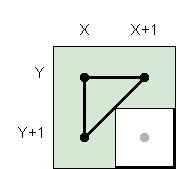
\includegraphics[width=\textwidth]{triangles-upper.pdf}
        \caption{Upper triangle.}
        \label{fig:triangle_generation:upper}
    \end{subfigure}
    % side-by-side
    \begin{subfigure}{0.3\textwidth}
        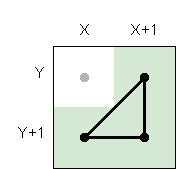
\includegraphics[width=\textwidth]{triangles-lower.pdf}
        \caption{Lower triangle.}
        \label{fig:triangle_generation:lower}
    \end{subfigure}
    % side-by-side
    \begin{subfigure}{0.3\textwidth}
        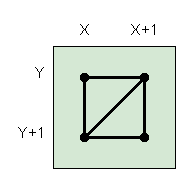
\includegraphics[width=\textwidth]{triangles-full.pdf}
        \caption{Both triangles.}
    \end{subfigure}
    
    \caption{Triangle creation. Green color indicates that the cell appears on occurrence map as visited.}
    \label{fig:triangle_generation}
\end{figure}

\begin{algorithm}
    \caption{Generating triangles using occurrence map.}

    \For{\textup{x} in 1..\textup{width}}{
        \For{\textup{y} in 1..\textup{width}}{
            \If{occuranceMap[x, y] and occuranceMap[x+1, y] and occuranceMap[x, y+1]}{
                recordTriangle(x, y, x+1, y, x, y+1)\;
            }
            \If{occuranceMap[x+1, y] and occuranceMap[x, y+1] and occuranceMap[x+1, y+1]}{
                recordTriangle(x+1, y, x, y+1, x+1, y+1)\;
            }
        }
    }
\end{algorithm}

Collected sets of vertices and triangles now form the mesh. Later, it is possible to apply some refinements to this mesh, e.g., texture, normals, or material data.

\subsection{Time complexity}

This algorithm executes two loops one after another: vertex grid building and triangles generation.

The first loop traverses over all chunk points. Thus, its complexity can be evaluated as $\mathcal{O}(n_1)$ (where $n_1$ is the number of points in a chunk), assuming that condition evaluation, math operations, and memory access have constant complexity.

The second loop traverses over the vertex grid, which has $length \times length$ cells. It means that its complexity can be evaluated as $\mathcal{O}(n_2)$ (where $n_2$ is the number of cells in a grid), assuming that other operations have constant complexity.

$$\mathcal{O}(n_1) + \mathcal{O}(n_2) = \mathcal{O}(n)$$
